\documentclass[dvipdfm]{book}

% % Package: geometry (formating PDF for kindle)
% \usepackage[
%     paperwidth=9cm, paperheight=12cm,
%     top=1cm, left=1cm, right=1cm, bottom=1.5cm,
%     includefoot
% ]{geometry}

% Package: hyperref (should be last package)
\usepackage{hyperref}
\hypersetup{
    bookmarks=true,
    pdftitle={OCEMR User Manual},
    pdfauthor={Carly J. Gielarowski},
    pdfproducer={Philip J. Freeman},
    pdfkeywords={ocemr} {manual},
    colorlinks=true,
}


\title{OCEMR User Manual}
\author{
    Carly J. Gielarowski\\
    $<$\href{mailto:joy.carly@gmail.com}{joy.carly@gmail.com}$>$
  \and
    Philip J. Freeman\\
    $<$\href{mailto:philip.freeman@gmail.com}{philip.freeman@gmail.com}$>$
}
\date{}
\begin{document}
\maketitle
\tableofcontents
\chapter{Getting Started}
\section{About this Manual}

In this section we will go over exactly what this manual intends to cover.

\subsection{Versions}
This manual covers OCEMR v0.4.X and superseeds previous documentation

While we attempt to mention all the differences between the versions
covered in this manual, there may be ommisions.

\section{About The Software}

% \subsection{Latest Informaion}


\subsection{Feature Requests and Bugs}
Feature requests and bugs can be submitted via the projects bugzilla site at
\url{https://bugs.kremlor.net/} or you can email the creator and maintainer
Philip Freeman $<$\href{mailto:philip.freeman@gmail.com}{philip.freeman@gmail.com}$>$.

\subsection{What's in a Browser}
TODO:

\section{Logging IN}
Once OCEMR is loaded in a supported browser, the
system will require the user to fill out the user name and password.
Every user has a unique user name and password. The user name and
password are both case sensitive. If a user originally used only lower
case letters when the user was first created, the user will only be
able to successfully log in to the system with lower case letters. In
order to log in to the system the user must enter the user name and
password and then click \textbf{Submit }or press the \textbf{Enter} key
on the keyboard.

\section{The Interface}
While logged in the main page of the user interface, the system
always has the same look and feel. 

\chapter{The User Interface}
\section{Introduction}

Introduce the overall flow of the system.

\section{Managing Patients}
\subsection{Finding a Patient}
\subsection{Adding a Patient}
\subsection{Patient Demographics}
\subsection{Patient Merge}

\section{The Patient Queue}

\section{The Patient's Visit}
\subsection{Allergies}
\subsection{Past Visits}
\subsection{Reason for Visit}
\subsection{Vitals / Exam}
\subsubsection{Vitals}
\subsubsection{Exam Notes}
\subsection{Labs}
\subsection{Assessment / Plan}
\subsection{Meds}
\subsection{Referrals}
\subsection{Immunizations}
\subsection{Notes}
\subsection{Finishing a Visit}

\section{The Lab Queue}

\section{The Med Queue}


\chapter{Administration}
This Chapter will explain in detail how to manage your OCEMR system.

\section{Introduction}

Managing users will be done through the application’s admin interface.
The admin interface can be extremely powerful and helpful, but also
dangerous. Please be careful while using it and follow the instructions
outlined here. Contact your system administrator or help desk person if
you have any questions.

\subsection{Relational Database Warning}

  OCEMR has, at it’s heart, a relational database that stores information
in an efficient and streamlined manner. When one piece of information in
the database refers to another, like when a Diagnosis is added for a Patient,
rather than store a copy of the patient’s name, the database store a reference
to that patient record. In most cases this is extremely helpful. Like if we
realize two visit’s in that patient’s name is spelled wrong. We edit the
patient’s name once and everywhere that record is referenced after that the
new name will appear.

  However, this can have drastic complications. Say, for instance, we delete
the patient we were talking about in the previous example. That patient is
referenced in all sorts of records throughout the system. All the notes,
symptoms, medication, diagnoses that were added refer back to that patient
record. Without the patient record, all those other records are
useless\footnote{in computer term they are ‘orphans’ because their
‘parents’ have disappeared} and will be deleted along with it.

\subsection{Navigating to the Admin Interface}

The admin interface is easy to find. When you have sufficient rights
to the interface, a link will appear in the main menu bar title \textbf{Admin}.
Just click it to enter the admin site.

  The admin interface looks like this:

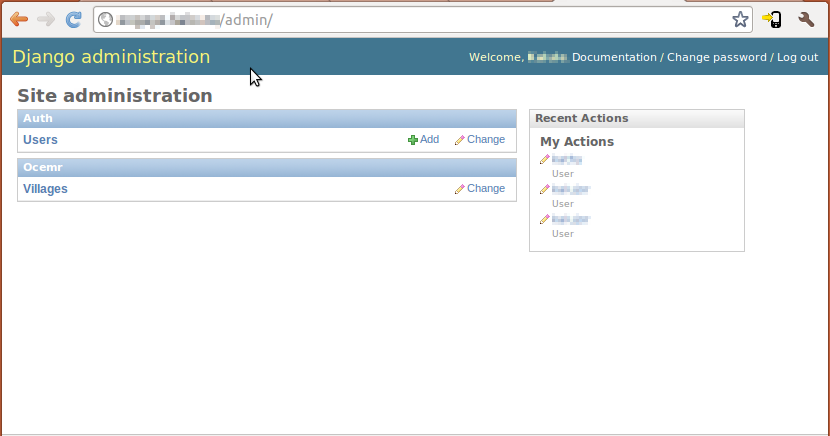
\includegraphics[keepaspectratio=true,width=\textwidth]{images/user_manual-administration/admin.png.eps}

\section{User Management}

\textbf{NEVER DELETE A USER FROM THE SYSTEM!} (Just disable the user instead.)

\subsection{Adding Users}
\subsubsection{Information Required}

  To add users you will need the following information:

\begin{enumerate}

\item Username

Select a username that is easy to remember for the user and also allows
everyone using the system to know who that name represents. \textbf{Usernames
should be all lowercase}.

\item Password

Tell the user to think of a password that they can remember and is not
easy for others to guess. The password can be reset at a later date by
anyone who has access to the user management functions of the admin
interface.

\item First and Last Name

The System will need this information especially when generating medical
records. It is important that this is added for the proper operation.

\item Email Address

In general it would be good practice to record a contact email address
here in case we need to get a hold of the user in the future or a place
to send login details or documentation.

\end{enumerate}

\subsubsection{Adding the User}
\begin{enumerate}
\item Click on \textbf{+Add} on the Main Admin page

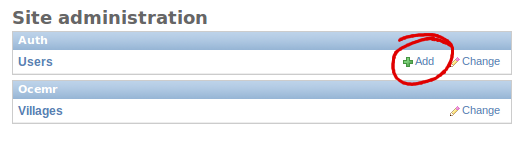
\includegraphics[keepaspectratio=true,width=\textwidth]{images/user_manual-administration/users-add_user.png.eps}

\item Enter the Username and Password, then click on Save.

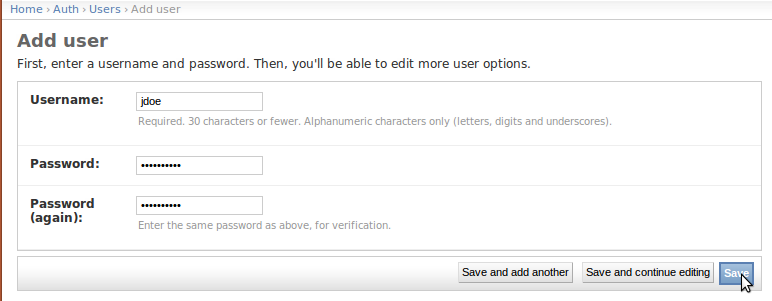
\includegraphics[keepaspectratio=true,width=\textwidth]{images/user_manual-administration/users-add_user_2.png.eps}

\item Next, Add the First Name, Last Name, and Email Address. Do NOT
Change any of the Permissions\footnote{Only Administrators need Staff status
and nobody should be given Superuser status. This will protect the
system from accidental data corruption.}!

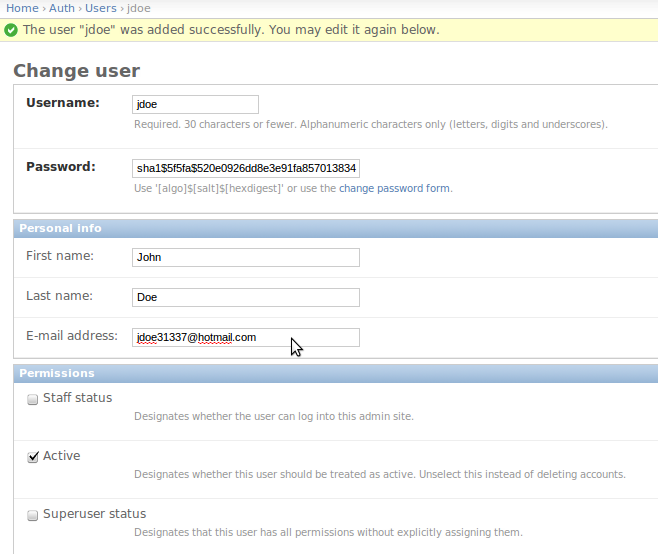
\includegraphics[keepaspectratio=true,width=\textwidth]{images/user_manual-administration/users-add_user_3.png.eps}

\item Scroll down to the bottom of the screen and click on \textbf{Save}.
\end{enumerate}

You will see the new user in the list.

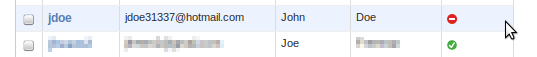
\includegraphics[keepaspectratio=true,width=\textwidth]{images/user_manual-administration/users-add_user_4.png.eps}

\subsection{Changing Passwords}

  The users currently do not have support for changing their own
passwords\footnote{This is slated for an upcoming release}, so as an
administrator for the system you may have to reset their password.

\begin{enumerate}
\item Click on \textbf{Change} from the Main Admin Page
\item Select the User you want to edit by clicking on the username.


\includegraphics[keepaspectratio=true,width=\textwidth]{images/user_manual-administration/users-select.png.eps}

\item Select \textbf{change password form}.

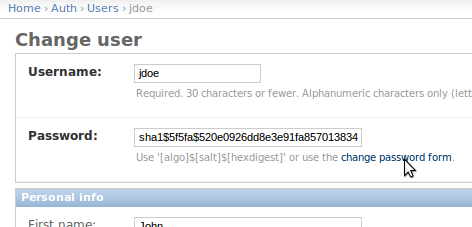
\includegraphics[keepaspectratio=true,width=\textwidth]{images/user_manual-administration/users-change_password.png.eps}

\item Enter the new password twice, and click \textbf{Change Password}.
\end{enumerate}

\subsection{Disabling Users}

  TODO: Explain when and why you should disable accounts.

\begin{enumerate}
\item Click on \textbf{Change} from the Main Admin Page
\item Select the User you want to edit by clicking on the username


\includegraphics[keepaspectratio=true,width=\textwidth]{images/user_manual-administration/users-select.png.eps}

\item Uncheck the \textbf{Active} box under permissions.
\item Scroll down to the bottom of the page and click \textbf{Save}.
\end{enumerate}


\appendix
\chapter{Hot Keys}
\section{Browser Shortcuts}

\end{document}
